% §4 The subordination bridge --- blueprint chapter 9 (blueprint/src/parts/09-bridge.tex),
% statements and proofs of record verbatim. Drafted 2026-09-15 from the blueprint at the state
% after the step-2 merges; prose rewritten 2026-09-17 at the author's review, on the six rules
% recorded at section 3 (notes/HANDOFF-article.md), plus the findings specific to this section:
%   - a motivation for the bridge in the context of scale-space theory (what later results need
%     it, what is for its own interest) and a map of the section at the head;
%   - a short informal introduction to the causal theory, so that the section reads without
%     the causal article at hand (4.1);
%   - the bridge on exponents expanded and emphasized as the construction of the section (4.2);
%     rem:bridge-route presented as an alternative route, not as "the route of the draft";
%   - 4.3-4.4 introduced by their results, not their proofs; a figure of the bridge on two corner
%     families (figures/fig-bridge.png from scripts/make-fig-bridge.py);
%   - the dimension filtration (4.5) motivated and then stated as a proposition with a proof:
%     the new blueprint node prop:dimension-filtration, [A] on the new ledger entry A23 (R166),
%     transcribed here with its page anchors before it; rem:dimension-filtration shortened to
%     what is a remark;
%   - the rest of the section given a structure: the witness lemma in a subsection of its own
%     (4.6), what crosses the bridge in another (4.7).
%
% This is the section where the causal article is MATHEMATICS rather than provenance (ADR-0003),
% so it is cited inside statements and proofs; no separate relation-to-the-causal-theory remark.
%
% Contents and departures from the blueprint chapter:
%   - all ten statement nodes transcribed under their markers: def:causal-admissible,
%     lem:bridge-exponents, prop:bridge-families, prop:bridge-strictness,
%     lem:subordinated-members, lem:student-subordinated, prop:dimension-filtration (the one [A]
%     node: ledger A23 with A2, A3, A7 read in dimension d; its page anchors are printed in the
%     prose before the statement, read from blueprint/AXIOMS.md), def:delay-data,
%     lem:filtration-strictness (notready: typed, sorry, the proof of record printed);
%   - rem:bridge-subordination, rem:bridge-route, rem:dimension-filtration and
%     rem:bridge-crossings are copied (remarks carry no marker); rem:bridge-subordination's
%     second paragraph and rem:bridge-route's framing are paper-side rewrites (2026-09-17, the
%     author's rule that the body carries no machine-checking talk), to be mirrored at the next
%     draft sync; rem:bridge-crossings' reference to the joint-locality theorem (module C) is a
%     sentence naming the next module's subject with no statement number and no promise;
%   - the blueprint's status annotations are not transcribed.

\section{The subordination bridge}\label{sec:bridge}

The causal theory of \sscite{fagerstrom2026hemigroup} classifies the scale spaces of a signal
in time, where a measurement may use the past and not the future, under the same weakening of
the semigroup to a hemigroup that the line paper applied in space. The two theories have the
same shape, and a classical construction connects them, Bochner's subordination
(\sscite{sato1999levy}, Theorem~30.1, p.~197).
Run a Brownian motion for a random time drawn from a causal kernel, and the displacement
reached has a symmetric law. This section makes that construction a map from the causal cone
into the admissible cone, family to family, and asks what it reaches.

\emph{Why the bridge.} Two later results need it, and one question is answered by it. The
Student-t family of \S\ref{sec:corners} is defined as the image of the causal Bessel corner,
and its properties are read off through the map; the exact implementation of the \Matern{}
family in \S\ref{sec:implementation} is the causal Gamma cascade carried across, its rational
transform becoming a rational spectrum. The question is which of the two theories is larger.
The bridge is injective, since a subordinated exponent determines its causal ancestor
(Proposition~\ref{prop:bridge-strictness}(1)), so the spatial theory contains a copy of the
causal one. It is not onto. The $\Cin$ rays of \S\ref{sec:cone}, and every member with no
Gaussian part whose profile is a lattice step, have no causal ancestor. So the symmetric
theory is strictly larger than the causal theory in Brownian disguise. The section then places
the image inside a chain of classes indexed by dimension, between the image and the cone, and
shows that the chain is strict at its bottom.

\emph{The map of the section.} \S\ref{sec:causal-brief} recalls the causal theory in the form
used here, one definition. \S\ref{sec:bridge-exponents} is the construction: on exponents the
bridge is a substitution, $F(\omega) = F_{\mathrm I}(\omega^2/2)$, and Lemma~\ref{lem:bridge-exponents}
says that it lands in the admissible cone and computes the profile of the image.
\S\ref{sec:bridge-families} lifts the map to families and follows the three causal corners
across (Proposition~\ref{prop:bridge-families}, Figure~\ref{fig:bridge}).
\S\ref{sec:bridge-strictness} proves that the map is not onto and says which members of the
image are the named families (Proposition~\ref{prop:bridge-strictness} and two lemmas).
\S\ref{sec:filtration} measures the gap between the image and the cone by a chain of classes
indexed by dimension (Proposition~\ref{prop:dimension-filtration}), \S\ref{sec:witness} gives
the one explicit family that shows the chain is strict at the bottom
(Lemma~\ref{lem:filtration-strictness}), and \S\ref{sec:crossings} lists what else of the causal
theory crosses. Throughout, $\BM$ is a standard Brownian motion, so
$\mathbb{E}\cos(\omega \BM_u) = e^{-u\omega^2/2}$, and $g_u$ is its law at time $u$, with
$g_0 = \delta_0$; a different diffusion constant is a change of spatial gauge and is not tracked.

\subsection{The causal theory, in brief}\label{sec:causal-brief}

The causal article axiomatizes the measurement of a temporal signal at every scale at once, on
the same pattern as \S\ref{sec:axioms-recap}. The operators are linear and positive, they form
a two-parameter hemigroup in scale, and they are continuous and scale covariant. In place of
translation and reflection covariance in space they have translation covariance in time
together with causality: the output at a time depends on the input up to that time only.

Its characterization theorem (\sscite{fagerstrom2026hemigroup}, Theorem~7.3) is the twin of
Theorem~\ref{thm:main-characterization}. An admissible causal family is, in its canonical
gauge, a family of convolutions by laws on the half-line. The kernel at scale $x$ is the law
of $x\,T_1$ for one random delay $T_1 \ge 0$, and the delays that occur are exactly the
self-decomposable laws on the half-line.

The dictionary between the two theories is short. Where a law on the line is described by its
cosine transform and an exponent $F$, a law on the half-line is described by its Laplace
transform and a Laplace exponent, $\mathbb{E}e^{-\sigma T_1} = e^{-F_{\mathrm I}(\sigma)}$. The
self-decomposable delays are those whose exponent is of the form below: a drift $b_0$, the
deterministic part of the delay, plus a catalogue of random delays of every size $u$ arriving
at rate $k_{\mathrm I}(u)\,du/u$, with $k_{\mathrm I}$ nonincreasing. This is the form of
\S\ref{sec:exponents-recap} with $1 - e^{-\sigma u}$ in place of $1 - \cos\omega x$. The
Gaussian coefficient $a$ of the line has the drift $b_0$ as its counterpart, and the folded
profile $k$ has the delay profile $k_{\mathrm I}$. The causal theory has three named corners.
The Gamma family has exponent $\gamma\log(1 + \sigma)$ and the Gamma laws as kernels. The
Bessel family has inverse-gamma laws as kernels, and its scale evolution is a local equation.
The stable family is the semigroup case.

One word of the definition needs a gloss. A \emph{Bernstein function} is a nonnegative smooth
function on $(0,\infty)$ whose derivative is completely monotone, that is whose derivatives
alternate in sign (\sscite{schilling2012bernstein}, Def.~3.1 and Thm.~3.2, p.~21). Except for
Proposition~\ref{prop:bridge-families}, which starts from a causal family, the statements of
this section read nothing of the causal axioms. What they read is the class of exponents,
recorded as a definition.

% shared with blueprint def:causal-admissible
\begin{definition}[the causal admissible cone]\label{def:causal-admissible}
A function $F_{\mathrm I} : [0,\infty) \to [0,\infty)$ is \emph{causally admissible} if
\[
  F_{\mathrm I}(\sigma) = b_0\,\sigma
   + \int_0^\infty \bigl(1 - e^{-\sigma u}\bigr)\,k_{\mathrm I}(u)\,\frac{du}{u},
  \qquad b_0 \ge 0, \quad k_{\mathrm I} : (0,\infty) \to [0,\infty) \ \text{nonincreasing},
\]
with $\int_0^1 k_{\mathrm I}(u)\,du < \infty$ and
$\int_1^\infty k_{\mathrm I}(u)\,u^{-1}du < \infty$. These are exactly the exponents the
time-causal article's characterization theorem attaches to its axioms, in its canonical gauge;
$(b_0, k_{\mathrm I})$ is its data, its drift and its delay profile. Such an
$F_{\mathrm I}$ is a Bernstein function vanishing at the origin, so $e^{-F_{\mathrm I}}$ is
completely monotone with value $1$ there; that it is therefore the Laplace transform of the law
of a random delay $T_1 \ge 0$ --- the subordination reading of this chapter --- is cited at
Remark~\ref{rem:bridge-subordination} and is not asserted here.
\end{definition}

The functions of the displayed form are Bernstein functions. Conversely every Bernstein
function vanishing at the origin has such a representation with a measure in place of
$k_{\mathrm I}(u)\,du/u$ (\sscite{schilling2012bernstein}, Thm.~3.2, p.~21). So what the
definition adds to being a Bernstein function is that the catalogue has a density and that
the density is nonincreasing, which is the self-decomposability of the delay. The two
integrability conditions are the causal counterpart of Lemma~\ref{lem:profile-integrability}.

\subsection{The bridge on exponents}\label{sec:bridge-exponents}

The construction of this section, in its simplest form, is a substitution. Take a causally
admissible exponent $F_{\mathrm I}$ and put
\[
  \Psi(\omega) := F_{\mathrm I}\bigl(\tfrac12\omega^2\bigr) .
\]
The reason this is the right substitution is the Brownian motion: its law at time $u$ has
cosine transform $e^{-u\omega^2/2}$, so replacing the Laplace variable $\sigma$ by
$\omega^2/2$ is what one gets by running $\BM$ for a random time $T_1$ and asking for the law of
the displacement, $\mathbb{E}\cos(\omega \BM_{T_1}) = \mathbb{E}e^{-T_1\omega^2/2}
= e^{-F_{\mathrm I}(\omega^2/2)}$. The lemma shows three things about $\Psi$. It is admissible,
that is of the form \ref{eq:sd-profile}: its Gaussian coefficient is
half the causal drift, and its folded profile is the delay catalogue seen through the Gaussian,
\[
  k(x) = 2x\int_0^\infty g_u(x)\,k_{\mathrm I}(u)\,\frac{du}{u} :
\]
a delay of size $u$ produces a Gaussian displacement of variance $u$, and the profile is the
mixture of these over the catalogue, folded onto the half-line. The profile is nonincreasing,
which is the one property not visible in that formula and is what makes the image
self-decomposable. And the law of $\BM_{T_1}$ is the law with exponent $\Psi$, which is what
justifies the name. The lemma states the three, with the delay entering the third as a
hypothesis (Remark~\ref{rem:bridge-subordination}).

% shared with blueprint lem:bridge-exponents
\begin{lemma}[the bridge on exponents]\label{lem:bridge-exponents}
Let $F_{\mathrm I}$ be causally admissible with data $(b_0, k_{\mathrm I})$ and put
\begin{equation}\label{eq:bridge}
  \Psi(\omega) := F_{\mathrm I}\bigl(\tfrac12\omega^2\bigr), \qquad \omega \in \RR .
\end{equation}
Then $\Psi$ is admissible in the sense of Theorem~\ref{thm:main-characterization}, that is of
the form \ref{eq:sd-profile}, with Gaussian coefficient $a = \tfrac12 b_0$ and folded profile
\begin{equation}\label{eq:bridge-profile}
  k(x) = 2x\int_0^\infty g_u(x)\,k_{\mathrm I}(u)\,\frac{du}{u}, \qquad x > 0,
\end{equation}
the Gaussian mixture of the delay catalogue. Moreover, if $T_1 \ge 0$ is a random delay
independent of $\BM$ with $\mathbb{E}e^{-\sigma T_1} = e^{-F_{\mathrm I}(\sigma)}$ for every
$\sigma \ge 0$, then the law of $\BM_{T_1}$ --- the mixture of the Gaussian laws against the law
of $T_1$ --- is a symmetric probability law with cosine transform $e^{-\Psi}$.
\end{lemma}

The construction is classical, and its two halves have different sources. The profile
\ref{eq:bridge-profile} is \sscite{sato2001subordination}'s (3.3), p.~8, in the two-sided
convention: his $k^{\sharp}(x) = x\int_0^\infty(2\pi s)^{-1/2}e^{-x^2/2s}\,k(s)\,ds/s$ is half
the folded profile above, and his (4.2)--(4.3), p.~9, record the same folding at the origin,
$k^{\sharp}(0{+}) = k(0{+})$ and $c_Y = 2c_Z$. That the image of a self-decomposable delay is
self-decomposable is \sscite{halgreen1979self}, \S3, p.~15, for a pure variance mixture, and
\sscite{sato2001subordination}, Theorem~1.1, for a general self-decomposable subordinator. What
this lemma adds is the form: it \emph{prescribes} the pair $(a,k)$ and checks it against the
requirements of \ref{eq:sd-profile} one by one, so that no representation theorem is spent and
the delay of the last clause is a hypothesis rather than something to be produced. The
monotonicity of the profile becomes visible after one substitution.

\begin{proof}
Write $\nu_2(x) = \int_0^\infty g_u(x)\,k_{\mathrm I}(u)\,du/u$ and $k(x) = 2x\,\nu_2(x)$, and
put $a = \tfrac12 b_0$. We verify that $(a,k)$ is a pair of the kind \ref{eq:sd-profile}
requires and that its exponent is $\Psi$; admissibility is then
Theorem~\ref{thm:main-characterization}.

\emph{$\nu_2$ is finite off the origin.} Fix $x \ne 0$. Below $u = 1$ the mixture integrand is
dominated by a multiple of $k_{\mathrm I}$: from $y^2 \le 4e^y$ at $y = x^2/2u$ we get
$e^{-x^2/2u} \le 16u^2/x^4$, and $u \le \sqrt{2\pi u}$ for $u \le 1$, so
$g_u(x)/u \le 16/x^4$ and the integrand is at most $(16/x^4)\,k_{\mathrm I}(u)$, integrable by
$\int_0^1 k_{\mathrm I} < \infty$. Above $u = 1$, $g_u \le 1$ and the integrand is at most
$k_{\mathrm I}(u)u^{-1}$, integrable by the second condition of
Definition~\ref{def:causal-admissible}. The two conditions pay in different places, and the
first pays only because of the Gaussian: the mixture carries $du/u$ where that condition
carries $du$, and the missing power of $u$ is supplied by the flatness of $g_u(x)$ as
$u \downarrow 0$ at a fixed $x \ne 0$.

\emph{$k$ is nonincreasing.} This is the clause that is not visible term by term. It becomes
visible in the right variable. Substituting $u = x^2v$, which leaves $du/u$ invariant,
\begin{equation}\label{eq:bridge-scaling}
  x\,\nu_2(x) = \int_0^\infty \frac{e^{-1/2v}}{v\sqrt{2\pi v}}\;k_{\mathrm I}(x^2v)\,dv ,
  \qquad x > 0 .
\end{equation}
The weight no longer involves $x$; the whole dependence sits in $k_{\mathrm I}(x^2v)$, which is
nonincreasing in $x > 0$ for each fixed $v > 0$ because $k_{\mathrm I}$ is nonincreasing. Hence
$k = 2x\nu_2(x)$ is nonincreasing on $(0,\infty)$.

\emph{The \Levy{} condition.} Since $\int_\RR (1 \wedge x^2)\,g_u(x)\,dx$ is at most the total mass
$1$ and at most the variance $u$, Tonelli gives
\[
  \int_0^\infty (1 \wedge x^2)\,k(x)\,\frac{dx}{x}
   = \int_0^\infty\Bigl(\int_\RR (1 \wedge x^2)\,g_u(x)\,dx\Bigr) k_{\mathrm I}(u)\,\frac{du}{u}
   \le \int_0^\infty (1 \wedge u)\,k_{\mathrm I}(u)\,\frac{du}{u} < \infty,
\]
the last integral being the single-integral reading of the two conditions of
Definition~\ref{def:causal-admissible}. By Lemma~\ref{lem:profile-integrability} this is the
pair of conditions \ref{eq:sd-profile} asks of $k$. So the spatial \Levy{} condition \emph{is}
the causal integrability condition, with the Gaussian performing the truncation.

\emph{The exponent.} Since $e^{-u\omega^2/2} = \int\cos(\omega x)\,g_u(x)\,dx$ and
$\int g_u = 1$, we have $1 - e^{-u\omega^2/2} = \int_\RR (1 - \cos\omega x)\,g_u(x)\,dx$, and
Tonelli gives
\[
  a\,\omega^2 + \int_0^\infty (1 - \cos\omega x)\,k(x)\,\frac{dx}{x}
   = \tfrac12 b_0\,\omega^2
     + \int_0^\infty \bigl(1 - e^{-u\omega^2/2}\bigr)\,k_{\mathrm I}(u)\,\frac{du}{u}
   = F_{\mathrm I}\bigl(\tfrac12\omega^2\bigr) = \Psi(\omega),
\]
the folding factor $2$ in $k = 2x\nu_2$ being exactly the factor the half-line reading of an
even integral needs.

\emph{The mixture reading.} Let $T_1 \ge 0$ be as in the statement. The mixture of the Gaussian
laws against the law of $T_1$ is a probability measure, each $g_u$ being one, and it is
symmetric, each $g_u$ being symmetric and symmetry passing through the mixture set by set.
Conditioning on $T_1$ and using $\mathbb{E}\cos(\omega \BM_u) = e^{-u\omega^2/2}$,
\[
  \mathbb{E}\cos(\omega \BM_{T_1}) = \mathbb{E}\,e^{-T_1\omega^2/2}
   = e^{-F_{\mathrm I}(\omega^2/2)} = e^{-\Psi(\omega)},
\]
the middle equality being the hypothesis read at $\sigma = \omega^2/2$. So the law of $\BM_{T_1}$
is a symmetric probability law with cosine transform $e^{-\Psi}$. Nothing here reads where the
delay law comes from: only its Laplace transform is used.
\end{proof}

% blueprint rem:bridge-subordination, copied; the two cited facts get their citekeys. Its second
% paragraph (what is and is not machine-checked) is reduced to one sentence paper-side
% (2026-09-17, the author's rule). NOT mirrored, deliberately (2026-09-19, R174): the blueprint
% records what is checked and why neither entry is admitted, and section 1.1 owns that account
% here (the author's decision D5).
\begin{remark}[the bridge is subordination]\label{rem:bridge-subordination}
A delay of the kind the lemma's second clause hypothesises always exists, and that is what makes
the bridge an instance of Bochner's subordination rather than a formal identity between
exponents. A causally admissible $F_{\mathrm I}$ is a Bernstein function vanishing at the
origin, so $e^{-F_{\mathrm I}}$ is completely monotone --- \sscite{schilling2012bernstein},
Thm.~3.7(iii) --- with value $1$ at the origin, and a completely monotone function with value
$1$ at the origin is the Laplace transform of a probability law on $[0,\infty)$ ---
\sscite{schilling2012bernstein}, Thm.~1.4, p.~3. That law is the law of a random delay
$T_1 \ge 0$, unique because a law on the half-line is determined by its Laplace transform, and
the lemma then says that the symmetric family attached to $\Psi$ is the family of laws of
$\BM_{T_1}$: Brownian motion run for the causal delay. The catalogue formula \ref{eq:bridge-profile}
is the same statement on profiles. Nothing in the paper depends on the two cited facts: every
consumer of the bridge quantifies over the delay law instead.
\end{remark}

% blueprint rem:bridge-route, copied; reframed paper-side (2026-09-17) as the alternative route
% it is, without the draft-versus-article history; MIRRORED in the blueprint 2026-09-19 (R174),
% which keeps the two ledger names and the sentence on which route is machine-checked (D5).
\begin{remark}[why the image is self-decomposable, in one line]\label{rem:bridge-route}
There is a second route to the admissibility clause, which produces the profile instead of
checking a prescribed one and shows in one line \emph{why} the image is self-decomposable. For
$c \in (0,1)$ the function $g = F_{\mathrm I} - F_{\mathrm I}(c^2\,\cdot)$ is again a Bernstein
function vanishing at the origin, so $e^{-\tau g}$ is completely monotone for every $\tau > 0$
and hence the Laplace transform of a probability law $\rho_\tau$ on $[0,\infty)$; then
$e^{-\tau(\Psi(\omega) - \Psi(c\omega))} = \int_{[0,\infty)} e^{-u\omega^2/2}\rho_\tau(du)$ is a
positive mixture of positive definite functions, so $\Psi - \Psi(c\,\cdot) \in \NDs$ for every
$c$, which is the self-decomposability condition of the line paper's
Lemma~\linenum{lem:selfdecomposable-exponents} and produces \ref{eq:sd-profile}. The route
rests on the two cited facts of the previous remark; the proof above rests on none, which is
why it is the proof of record.
\end{remark}

\subsection{The bridge on families, and the corners}\label{sec:bridge-families}

The map on exponents lifts to a map on families. Given a causal family in its canonical gauge,
mix its kernel from causal scale $s^2$ to causal scale $t^2$ against the Gaussian laws and
call the result the spatial kernel from $s$ to $t$. The proposition says that this is an
admissible family on the line, in canonical gauge, with exponent $F_{\mathrm I}(\omega^2/2)$,
and it follows the named members across:
\begin{itemize}
\item the causal pure delay becomes the Gaussian;
\item the Gamma family becomes the \Matern{} family;
\item the Bessel family becomes the Student-t family;
\item the stable family of index $\alpha$ becomes the symmetric stable family of index
$2\alpha$;
\item a causal scale $x$ becomes the spatial scale $\sqrt x$.
\end{itemize}
Figure~\ref{fig:bridge} shows two of the corners crossing.

% shared with blueprint prop:bridge-families
\begin{proposition}[the bridge on families; the corners; the gauges]\label{prop:bridge-families}
Let $(\Phi^{\mathrm I}_{x,y})$ be a time-causal family satisfying the causal axioms, with
kernels $\mu^{\mathrm I}_{x,y}$ on $[0,\infty)$ written in its canonical gauge and exponent
$F_{\mathrm I}$. Define, for $0 \le s \le t$,
\begin{equation}\label{eq:bridge-families}
  \mu_{s,t} := \int_{[0,\infty)} g_u\;\mu^{\mathrm I}_{s^2,t^2}(du),
  \qquad \Phis{s}{t}f := \mu_{s,t} * f .
\end{equation}
Then $(\Phis{s}{t})$ satisfies (A1)--(A8) and (ND) with $S_\lambda t = \lambda t$; the
coordinate $t$ is its canonical gauge, and its exponent is $F = F_{\mathrm I}(\cdot^2/2)$. In
particular:
\begin{enumerate}
\item the causal pure delay, $\mu^{\mathrm I}_{x,y} = \delta_{y-x}$, maps to the Gaussian family
of Proposition~\ref{prop:two-members}, $\mu_{s,t} = g_{t^2-s^2}$; the causal drift ray
$b_0\sigma$ maps to the Gaussian ray $\tfrac12 b_0\omega^2$;
\item the causal Gamma family, $F_{\mathrm I}(\sigma) = \gamma\log(1+\sigma)$, maps to the
\Matern{} family at range $1/\sqrt2$: $F(\omega) = \gamma\log(1 + \omega^2/2)$, folded profile
$k(x) = 2\gamma e^{-\sqrt2\,x}$;
\item if the inverse-gamma laws of shape $a$ are the delay kernels of such a family --- the causal
Bessel family, whose existence is cited at Remark~\ref{rem:student-ggc} and asserted nowhere here
--- then it maps to the Student-t family with $2a$ degrees of freedom. The mixture identity behind
that clause is unconditional: mixing the Gaussian kernels against the inverse-gamma law of shape
$a$ gives the Student-t law with $2a$ degrees of freedom, which is
Proposition~\ref{prop:student-t}(1);
\item the causal stable family, $F_{\mathrm I}(\sigma) = \sigma^\alpha$ with
$0 < \alpha \le 1$, maps to the symmetric stable family
$F(\omega) = 2^{-\alpha}|\omega|^{2\alpha}$ of index $2\alpha \in (0,2]$; the boundary
$\alpha = 1$ is item (1);
\item the spatial canonical gauge is the square root of the causal one: a causal scale $x$
becomes the spatial scale $t = \sqrt x$, which is the parabolic gauge of the causal article.
\end{enumerate}
\end{proposition}

% Figure: the bridge on two corner families (2026-09-17, the author's request at the review);
% the image is figures/fig-bridge.png from scripts/make-fig-bridge.py (numpy + matplotlib,
% closed forms, no data).
\begin{figure}[t]
\centering

\includegraphics[width=\textwidth]{fig-bridge.png}
\caption{The bridge on two corners, at canonical scale $1$. Left, the causal kernel: the law
of the delay $T_1$ on the half-line. Right, its image: the law of $\BM_{T_1}$, Brownian motion run
for that delay, on the line. Top row, the causal Gamma family at $\gamma = 2$, delay density
$u\,e^{-u}$, whose image is the \Matern{} member of index $2$ at range $1/\sqrt2$
(Proposition~\ref{prop:bridge-families}(2)); the exponents are related by the substitution
$\sigma = \omega^2/2$ and the profiles by the Gaussian mixture \ref{eq:bridge-profile}. Bottom
row, the causal Bessel family at shape $a = \tfrac32$, the inverse-gamma delay $T_1 = 1/V$
with $V$ chi-square on $3$ degrees of freedom, whose image is the Student-t member with $3$
degrees of freedom in the scale of Proposition~\ref{prop:student-t}, with density
$(2/\pi)(1+x^2)^{-2}$ (clause (3)). The heavy tail of the delay
becomes the heavy tail of the displacement.}
\label{fig:bridge}
\end{figure}

The proof has one step beyond Lemma~\ref{lem:bridge-exponents}, the identification of the
mixtures \ref{eq:bridge-families} with the kernels the characterization theorem attaches to
$F$, and the corners are then computations on profiles and exponents; item (2) is computed
from the causal \emph{profile}, so that the Gamma exponent comes out rather than going in.

\begin{proof}
\emph{The family.} $\hat\mu_{s,t}(\omega) = \int e^{-u\omega^2/2}\,\mu^{\mathrm I}_{s^2,t^2}(du)
= \widehat{\mu^{\mathrm I}_{s^2,t^2}}(\omega^2/2)
= \exp[-(F_{\mathrm I}(t^2\omega^2/2) - F_{\mathrm I}(s^2\omega^2/2))]$, using the causal
similarity form in the canonical gauge. So $g_{s,t}(\omega) = F(t\omega) - F(s\omega)$ with
$F = F_{\mathrm I}(\cdot^2/2)$, admissible by Lemma~\ref{lem:bridge-exponents}; the family is
therefore the one Theorem~\ref{thm:main-characterization} attaches to $F$ in the canonical
gauge, and that construction verified (A1)--(A8) and (ND), with $S_\lambda t = \lambda t$ because
$F(\lambda t\omega) - F(\lambda s\omega) = g_{s,t}(\lambda\omega)$. Directly:
$\Dil{\lambda}g_u = g_{\lambda^2u}$, so a spatial dilation by $\lambda$ is a causal dilation by
$\lambda^2$, and the causal covariance
$\Dil{\lambda^2}\mu^{\mathrm I}_{x,y} = \mu^{\mathrm I}_{\lambda^2x,\lambda^2y}$ becomes
$\Dil{\lambda}\mu_{s,t} = \mu_{\lambda s,\lambda t}$; the cascade is inherited from the
independent increments of both $\BM$ and the delay.

Two identifications in that paragraph need justification, and they are where the work is
once Lemma~\ref{lem:bridge-exponents} is in hand. First, the kernels
Theorem~\ref{thm:main-characterization} attaches to $F$ and the mixtures
\ref{eq:bridge-families} are \emph{a priori} two different families; they agree because both
are symmetric probability measures and their cosine transforms agree, so
Proposition~\ref{prop:fourier-uniqueness} identifies them. Second, the scaling action is
$S_\lambda t = \lambda t$ on the nose, not merely up to the gauge: the construction of
Theorem~\ref{thm:main-characterization} produces the gauge conjugate
$\chi^{-1}(\lambda\chi(t))$, which in the canonical gauge $\chi = \mathrm{id}$ is $\lambda t$
for every $t \ge 0$, and every clause of (A8) reads $S_\lambda$ on $[0,\infty)$ only.

(1) $\mu^{\mathrm I}_{x,y} = \delta_{y-x}$ gives $\mu_{s,t} = g_{t^2-s^2}$, and
$F_{\mathrm I}(\sigma) = b_0\sigma$ gives $F(\omega) = \tfrac12 b_0\omega^2$.

(2) Take the causal Gamma family by its \emph{profile}, $k_{\mathrm I}(u) = \gamma e^{-u}$ with
no drift; the exponent then comes out of the computation rather than into it. By
\ref{eq:bridge-profile} the image has folded profile
\[
  k(x) = 2\gamma x\int_0^\infty g_u(x)\,e^{-u}\,\frac{du}{u}
       = \frac{2\gamma x}{\sqrt{2\pi}}\int_0^\infty u^{-3/2}e^{-x^2/2u}e^{-u}\,du
       = 2\gamma e^{-\sqrt2\,x},
\]
by the identity $\int_0^\infty u^{-3/2}e^{-A/u - Bu}\,du = \sqrt{\pi/A}\,e^{-2\sqrt{AB}}$ at
$A = x^2/2$, $B = 1$ --- equivalently, the Laplace transform
$\int_0^\infty \frac{x}{\sqrt{2\pi u^3}}e^{-x^2/2u}e^{-\sigma u}du = e^{-x\sqrt{2\sigma}}$ of the
first-passage law of Brownian motion at level $x$, at $\sigma = 1$. That is the folded profile
$2\gamma e^{-x/t}$ of Proposition~\ref{prop:matern-exponent} at $t = 1/\sqrt2$. The exponent now
follows without a second integral: \ref{eq:bridge} says that $F_{\mathrm I}(\omega^2/2)$
\emph{is} the exponent of the admissible datum whose folded profile is
\ref{eq:bridge-profile}, and that profile has just been identified, so
Proposition~\ref{prop:matern-exponent}(1) evaluates it and
$F(\omega) = \gamma\log(1 + \omega^2/2) = \gamma\log(1 + t^2\omega^2)$ at $t = 1/\sqrt2$. In
particular the causal exponent $\gamma\log(1+\sigma)$ is a consequence of the causal profile and
need not be assumed.

(3) is the classical normal variance-mixture representation, computed in
Proposition~\ref{prop:student-t}(1); that identity needs no hypothesis on the causal side. Under
the clause's hypothesis --- that the inverse-gamma law of shape $a$ is the delay law of a causally
admissible $F_{\mathrm I}$ --- Lemma~\ref{lem:bridge-exponents} makes the image admissible and
self-decomposable, and Lemma~\ref{lem:student-subordinated} is the same statement read as
membership in $\mathcal{S}$.

(4) $(\omega^2/2)^\alpha = 2^{-\alpha}|\omega|^{2\alpha}$, and $\alpha \le 1$ maps onto index
at most $2$.

(5) The causal accumulated exponent in the canonical gauge is $F_{\mathrm I}(x\sigma)$, and the
image has $\hat\mu_{0,t}(\omega) = e^{-F_{\mathrm I}(t^2\omega^2/2)} = e^{-F(t\omega)}$, so the
spatial gauge $t$ satisfies $t^2 = x$.
\end{proof}

The causal article names its parabolic gauge because in it
the memory-line evolution of its Bessel family is a Bessel operator, a heat-type generator; the
reason is now visible from the other side, that parameter being the spatial scale of the
subordinated family, with the factor $\tfrac12$ from Brownian scaling. The two articles'
natural coordinates agree through $x = t^2$, causal scale being a variance and spatial scale a
standard deviation --- which is also why the scale-space literature's diffusion variable is the
square of this paper's $t$ (Remark~\ref{rem:gauge-freedom}).

\subsection{Strictness: the bridge is not onto}\label{sec:bridge-strictness}

The image of the bridge is a subcone of the admissible cone, and the proposition says what
separates it from the whole: a subordinated exponent is strictly increasing on the half-line,
because it is a Bernstein function of $\omega^2$, whereas an admissible exponent may have
stationary points, and exactly the ones with no Gaussian part whose profile is a step function with all its jumps
on a lattice do. The $\Cin$ rays are the simplest case, one jump. So the extreme rays of the
cone, other than the Gaussian, have no causal ancestor, and the image is strictly smaller than
the cone. The two lemmas that follow say which named families do lie in the image: the
Gaussian ray and the \Matern{} and stable families unconditionally, and the Student-t family
under a hypothesis on its delay law that the literature supplies.

% shared with blueprint prop:bridge-strictness
\begin{proposition}[strictness: the bridge is not onto]\label{prop:bridge-strictness}
Call an admissible $F$ \emph{subordinated} if $F(\omega) = F_{\mathrm I}(\omega^2/2)$ for some
causally admissible $F_{\mathrm I}$, and write $\mathcal{S}$ for the set of subordinated
exponents.
\begin{enumerate}
\item $F$ is subordinated if and only if $\sigma \mapsto F(\sqrt{2\sigma})$ is causally
admissible.
\item Every subordinated $F$ other than $0$ is strictly increasing on $(0,\infty)$, with
$F' > 0$ there.
\item No $\Cin$ ray is subordinated, since $\Cin'(z) = (1 - \cos z)/z$ vanishes at every
$z \in 2\pi\ZZ \setminus \{0\}$. More generally, an admissible $F$ has a stationary point
$\omega_0 \ne 0$ if and only if $a = 0$ and the Choquet measure $\varpi$ of
Proposition~\ref{prop:choquet-cone} is carried by the lattice $\tfrac{2\pi}{|\omega_0|}\ZZ$,
that is, if and only if $a = 0$ and the profile $k$ is a step function with all its jumps on that lattice;
and no such $F$ with $F \not\equiv 0$ is subordinated.
\item $\mathcal{S}$ is a convex subcone of the admissible cone, closed under the dilations
$F \mapsto F(\lambda\,\cdot)$; it contains none of the extreme rays $\Cin(\tau\,\cdot)$.
\end{enumerate}
\end{proposition}

\begin{proof}
(1) is Definition~\ref{def:causal-admissible} read on $F_{\mathrm I}(\sigma) := F(\sqrt{2\sigma})$.

(2) Let $F = F_{\mathrm I}(\cdot^2/2)$ with $F_{\mathrm I}$ causally admissible, and suppose
$F \not\equiv 0$. Fix $\sigma > 0$. On $(1,\infty)$ the elementary bound
$u\,e^{-\sigma u/2} \le 2/\sigma$ turns $e^{-\sigma u/2}k_{\mathrm I}(u)$ into
$(2/\sigma)\,k_{\mathrm I}(u)u^{-1}$, integrable by the second condition of
Definition~\ref{def:causal-admissible}, and on $(0,1)$ it is at most $k_{\mathrm I}$, integrable
by the first; so $e^{-\sigma u/2}k_{\mathrm I}(u)$ dominates the $\sigma$-derivative
$e^{-\sigma u}k_{\mathrm I}(u)$ of the integrand uniformly for $\sigma$ in a neighbourhood of
the given one, and differentiation under the integral sign gives
\[
  F_{\mathrm I}'(\sigma) = b_0 + \int_0^\infty e^{-\sigma u}\,k_{\mathrm I}(u)\,du,
  \qquad \sigma > 0 .
\]
Both terms are nonnegative. If the sum vanishes at one $\sigma > 0$ then $b_0 = 0$ and, the
exponential being strictly positive, $k_{\mathrm I} = 0$ almost everywhere on $(0,\infty)$;
but then the representation makes $F_{\mathrm I}$, and so $F$, identically zero. Hence
$F_{\mathrm I}' > 0$ on $(0,\infty)$, and the chain rule gives
$F'(\omega) = \omega\,F_{\mathrm I}'(\omega^2/2) > 0$ for $\omega > 0$. A function continuous
on $(0,\infty)$ with positive derivative there is strictly increasing there, and $F$ is
continuous, its representation \ref{eq:sd-profile} being so by dominated convergence.

The derivative formula is the only place the causal representation is differentiated, and one
classical step does \emph{not} enter it. Read as a function of $\sigma$, $F_{\mathrm I}'$ is
the Laplace transform of the positive measure $b_0\delta_0 + k_{\mathrm I}(u)\,du$, so it is
completely monotone and one may argue, as the causal article does, that a completely monotone
function vanishing at an interior point vanishes identically. That is Bernstein's theorem, and
it is not needed: it \emph{produces} a representing measure, and
Definition~\ref{def:causal-admissible} has already given one. What is left is the positivity of
an integral, which is the display above.

(3) $\Cin'(2\pi n) = 0$ for every nonzero integer $n$, which contradicts (2); so no $\Cin$ ray
is subordinated. For the general statement, \ref{eq:symbol} gives
$\omega F'(\omega) = B(\omega) = 2a\omega^2 + \int (1 - \cos\omega u)\,\varpi(du)$, a sum of
nonnegative terms, which vanishes at $\omega_0 \ne 0$ if and only if $a = 0$ and
$\cos(\omega_0 u) = 1$ for $\varpi$-almost every $u$; the latter says, by the argument of
Lemma~\ref{lem:lattice-zero} applied to $\varpi$, that $\varpi$ is carried by
$\tfrac{2\pi}{|\omega_0|}\ZZ$, which is the profile $k = \varpi((\cdot,\infty))$ being a step
function with jumps on that lattice. Such an $F$ has a stationary point off the origin, so it
is not subordinated, by (2).

(4) $\mathcal{S}$ is the image of the causal cone under $F_{\mathrm I} \mapsto
F_{\mathrm I}(\cdot^2/2)$, so the three closure properties are closure properties of the causal
cone, and the map carries them across because it is linear and because
$F_{\mathrm I}(\lambda^2\,\cdot)$ maps to $F(\lambda\,\cdot)$ --- a spatial dilation by
$\lambda$ is a causal dilation by $\lambda^2$. On the causal side, sums and nonnegative
multiples act on the data $(b_0, k_{\mathrm I})$ termwise and the two conditions of
Definition~\ref{def:causal-admissible} are preserved term by term. The dilation
$F_{\mathrm I} \mapsto F_{\mathrm I}(c\,\cdot)$, $c > 0$, has data
$(c\,b_0, k_{\mathrm I}(\cdot/c))$, and for it the two conditions are better read as the single
one
\[
  \int_0^\infty (1 \wedge u)\,k_{\mathrm I}(u)\,\frac{du}{u} < \infty,
\]
which they are equivalent to, $(1 \wedge u)/u$ being $1$ below $1$ and $u^{-1}$ above it. The
change of variables $u = cx$ leaves $du/u$ invariant, so it transforms that integral into
$\int_0^\infty (1 \wedge cx)\,k_{\mathrm I}(x)\,dx/x$, and
$1 \wedge cx \le \max(1,c)\,(1 \wedge x)$ bounds it by $\max(1,c)$ times the undilated one.
Splitting the two windows first would instead require the change of variables on two moving
intervals. The exclusion of the $\Cin$ rays is (3), whose Choquet coordinates are
Proposition~\ref{prop:choquet-cone}.
\end{proof}

The next lemma exhibits a causal ancestor for each of three named families.

% shared with blueprint lem:subordinated-members
\begin{lemma}[the subordinated slice's members]\label{lem:subordinated-members}
$\mathcal{S}$ contains the Gaussian ray and the \Matern{} and symmetric stable families.
\end{lemma}

\begin{proof}
Membership in $\mathcal{S}$ asks for a causally admissible datum $(b_0, k_{\mathrm I})$ whose
exponent, read at $\omega^2/2$, is the given exponent. One datum is exhibited per family, and the
named families at their general parameters are then reached by the closure clauses of
Proposition~\ref{prop:bridge-strictness}(4).

\emph{The Gaussian ray.} For $b_0 \ge 0$ the datum $(b_0, 0)$ satisfies
Definition~\ref{def:causal-admissible} with nothing to check, and its exponent is
$F_{\mathrm I}(\sigma) = b_0\sigma$ for $\sigma \ge 0$. With $b_0 = 2a$ it gives
$F_{\mathrm I}(\omega^2/2) = a\omega^2$.

\emph{The \Matern{} family.} Let $b_0 = 0$ and $k_{\mathrm I}(u) = \gamma e^{-u}$ for $u > 0$. The
profile is nonincreasing, bounded by $\gamma$ on $(0,1)$, and $k_{\mathrm I}(u)/u \le \gamma
e^{-u}$ on $(1,\infty)$, so both conditions of Definition~\ref{def:causal-admissible} hold. By
Proposition~\ref{prop:bridge-families}(2), $F_{\mathrm I}(\omega^2/2) = \gamma\log(1 +
\omega^2/2)$, the \Matern{} exponent at range $1/\sqrt2$. For $\theta > 0$,
\[
  \gamma\log(1 + \theta^2\omega^2) = \gamma\log\bigl(1 + \tfrac12(\sqrt2\,\theta\,\omega)^2\bigr),
\]
so the \Matern{} exponent at range $\theta$ is the dilation by $\lambda = \sqrt2\,\theta$ of the one
at range $1/\sqrt2$, and it lies in $\mathcal{S}$ because $\mathcal{S}$ is closed under
dilations.

\emph{The symmetric stable family.} Let $0 < \beta < 1$ and $c_\beta = \beta/\Gamma(1-\beta)$,
and take $b_0 = 0$ and $k_{\mathrm I}(u) = c_\beta u^{-\beta}$ for $u > 0$. The profile is
nonincreasing, and $\int_0^1 u^{-\beta}du = (1-\beta)^{-1}$ and
$\int_1^\infty u^{-\beta-1}du = \beta^{-1}$ are finite, the first because $\beta < 1$ and the
second because $\beta > 0$. Its exponent is
\[
  F_{\mathrm I}(\sigma) = \sigma^\beta, \qquad \sigma \ge 0 .
\]
The profile is homogeneous: $k_{\mathrm I}(u/c) = c^\beta k_{\mathrm I}(u)$ for $c > 0$. So the
dilated datum $(c\,b_0, k_{\mathrm I}(\cdot/c))$ of the proof of
Proposition~\ref{prop:bridge-strictness}(4), whose exponent is $F_{\mathrm I}(c\,\cdot)$, is the
datum $(c^\beta b_0, c^\beta k_{\mathrm I})$, whose exponent is $c^\beta F_{\mathrm I}$; hence
$F_{\mathrm I}(\sigma) = \sigma^\beta F_{\mathrm I}(1)$ for every $\sigma > 0$. The two sides
agree on a neighbourhood of $\sigma = 1$, so their derivatives there agree: the right side has
derivative $\beta F_{\mathrm I}(1)$, and by the derivative formula in the proof of
Proposition~\ref{prop:bridge-strictness}(2)
\[
  F_{\mathrm I}'(1) = \int_0^\infty e^{-u}\,c_\beta u^{-\beta}\,du = c_\beta\,\Gamma(1-\beta)
  = \beta .
\]
Hence $F_{\mathrm I}(1) = 1$, and $F_{\mathrm I}(0) = 0$ by the representation. By
Proposition~\ref{prop:bridge-families}(4), $F_{\mathrm I}(\omega^2/2) = 2^{-\beta}|\omega|^{2\beta}$.
Given $0 < \alpha < 2$, take $\beta = \alpha/2$: then
$|\omega|^\alpha = 2^{\alpha/2}F_{\mathrm I}(\omega^2/2)$ is a positive multiple of a member of
$\mathcal{S}$, and lies in $\mathcal{S}$, which is a cone.
\end{proof}

For the Student-t family the delay is the inverse-gamma law, and what has to be known is that
this law is the delay law of a causally admissible exponent, that is that it is
self-decomposable on the half-line. That is a theorem of Halgreen's
(\sscite{halgreen1979self}, \S2, pp.~14--15, recorded as Remark~\ref{rem:student-ggc}). The
lemma takes it as a hypothesis and proves the membership from it.

% shared with blueprint lem:student-subordinated
\begin{lemma}[the Student-t family is subordinated]\label{lem:student-subordinated}
Let $a > 0$, let $T_1$ be the inverse-gamma law of shape $a$ of
Proposition~\ref{prop:student-t}, and suppose $T_1$ is the delay law of a causally admissible
exponent: that for some $F_{\mathrm I}$ as in Definition~\ref{def:causal-admissible},
\[
  \mathbb{E}e^{-\sigma T_1} = e^{-F_{\mathrm I}(\sigma)}, \qquad \sigma \ge 0 .
\]
Then $\mathcal{S}$ contains the Student-t family of shape $a$, with $F_{\mathrm I}$ as its causal
ancestor. That $T_1$ is such a delay law is cited at Remark~\ref{rem:student-ggc} and is not
asserted here.
\end{lemma}

\begin{proof}
Conditioning the Brownian kernel on $T_1$, the Student-t law of shape $a$ is the mixture of the
Gaussian laws against the law of $T_1$ --- Proposition~\ref{prop:bridge-families}(3) --- so its
cosine transform at $\omega$ is $\mathbb{E}e^{-T_1\omega^2/2}$, which is the mixture identity of
Lemma~\ref{lem:bridge-exponents}. The hypothesis read at $\sigma = \omega^2/2$ turns that into
$e^{-F_{\mathrm I}(\omega^2/2)}$. So an exponent $F$ of the Student-t family --- one with
$e^{-F(\omega)} = \hat\phi_1(\omega)$ at every frequency --- satisfies
$e^{-F(\omega)} = e^{-F_{\mathrm I}(\omega^2/2)}$ there, hence
$F(\omega) = F_{\mathrm I}(\omega^2/2)$ pointwise, the exponential being injective. That is
membership in $\mathcal{S}$, with $F_{\mathrm I}$ as the ancestor.
\end{proof}

The criterion in clause (3) of Proposition~\ref{prop:bridge-strictness} is the second
appearance of one phenomenon. The first is in the line paper. A zero of an \emph{exponent} at
$\omega_0 \ne 0$ means that the law is carried by the lattice $\tfrac{2\pi}{\omega_0}\ZZ$
(Lemma~\ref{lem:lattice-zero}), and scale covariance excludes such laws
(Lemma~\ref{lem:no-lattice}). Here a zero of the \emph{symbol} $\omega F'$ at $\omega_0 \ne 0$
means a lattice \emph{profile}, a step function whose jumps lie on a lattice, that is a tail
measure $\varpi$ carried by the lattice, and no axiom excludes it. The $\Cin$ rays are the
case of a single step. What excludes it is subordination, because a Gaussian mixture spreads
every delay over the whole line.

Symmetric self-decomposable laws with a lattice-step profile are therefore members of the
spatial theory with no causal ancestor. The converse --- that a member with no causal ancestor
must have a step profile --- is not asserted, and it fails: an admissible $F$
whose \emph{tail measure} $\varpi = -dk$ is carried by a compact subset of $(0,\infty)$ and has no
atom there, equivalently whose profile is continuous and of bounded support,
has no ancestor either, because a subordinated profile is a Gaussian mixture of the delay
catalogue (\ref{eq:bridge-profile}) and is therefore positive at every $x > 0$. (The catalogue
itself is carried by no compact subset of $(0,\infty)$: a nonincreasing $k \not\equiv 0$ is
positive on a neighbourhood of the origin.) The next two
subsections place $\mathcal{S}$ inside a chain of larger classes.

\subsection{The dimension filtration}\label{sec:filtration}

Clause (1) of Proposition~\ref{prop:bridge-strictness} turns membership of $\mathcal{S}$ into a
condition on one function of one variable: $F$ is subordinated exactly when
$\sigma \mapsto F(\sqrt{2\sigma})$ is causally admissible. Definition~\ref{def:causal-admissible}
asks two things of that function, that it be a Bernstein function vanishing at the origin and
that its delay profile be nonincreasing, and dropping the second leaves a condition with a
geometric meaning. A theorem of Schoenberg's, the \emph{radial theorem}, says, up to a dilation
of $\xi$ that changes nothing, that
$f(\sigma) = F(\sqrt{2\sigma})$ is a Bernstein function exactly when the radial extension
$\xi \mapsto F(|\xi|)$ is a \Levy{} exponent on $\RR^d$ for every dimension $d$ at once. So the
larger class is the set of line exponents that are radial profiles of isotropic infinitely
divisible laws in every dimension, and the question how far $\mathcal{S}$ is from the
admissible cone can be asked dimension by dimension: for which $d$ is $F(|\xi|)$ the exponent
of a self-decomposable law on $\RR^d$? This is the natural question for a scale-space theory,
since the isotropic scale spaces of the plane and of space have kernels of exactly that form,
and their restrictions to a line are members of the line's theory: the classes below are,
heuristically, the exponents that come from an isotropic admissible family in dimension $d$.
The proposition says that the classes form a chain, that the image of the bridge sits at the
bottom of every one of them, that the lattice-step members with no Gaussian part lie
outside their intersection, and that the intersection is exactly the image of the bridge. Figure~\ref{fig:filtration} draws the chain with what is known
about it and what is not.

% Figure: the dimension filtration as nested regions. Referenced from section 4.5 before
% prop:dimension-filtration. Pure TikZ, schematic (2026-09-19; redrawn the same day after the
% external review: clause (4) gives A_infty = S, so the innermost region is one region, and the
% presentation review asked that the geometry assert no membership the text does not). It draws
% what prop:dimension-filtration and lem:filtration-strictness establish: the chain
% A_1 > A_2 > A_3 > ... > A_infty = S, the two witnesses F^(8) in A_1 \ A_2 and F^(4) in
% A_2 \ A_3, and the class B around A_infty with the Cin rays outside it. What is not
% established is said in words inside the figure: nothing is claimed about B against the finite
% A_d, so B is drawn as a dashed contour and the Cin rays are placed outside B only, in a box
% that says so.

\begin{figure}[t]
\centering
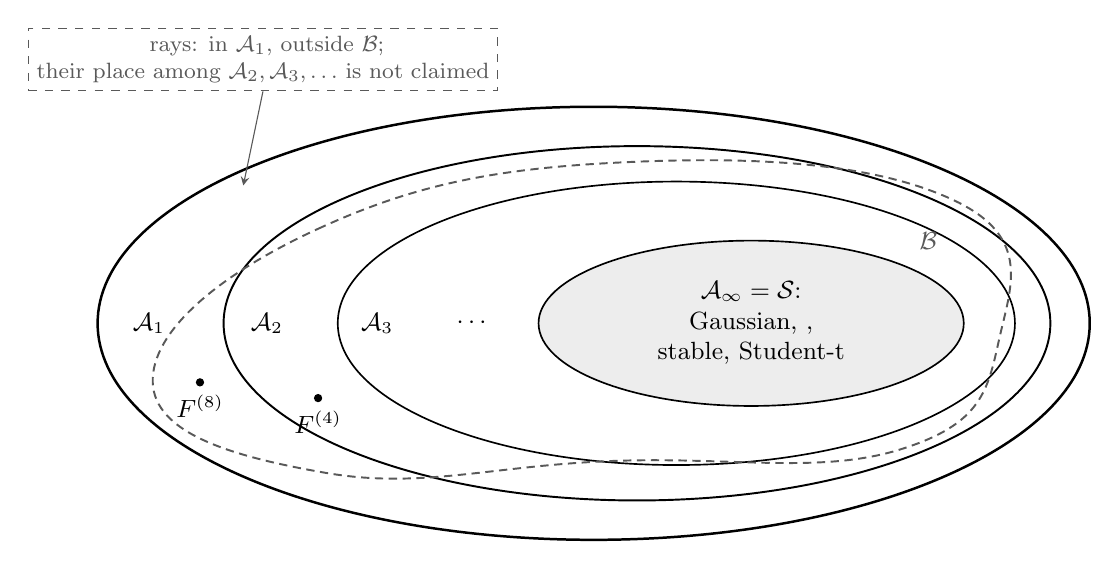
\begin{tikzpicture}[every node/.style={font=\small}, >=stealth]
% the chain
\draw[line width=0.9pt] (0,0) ellipse [x radius=6.3, y radius=2.75];
\draw[line width=0.7pt] (0.55,0) ellipse [x radius=5.25, y radius=2.25];
\draw[line width=0.6pt] (1.05,0) ellipse [x radius=4.3, y radius=1.8];
\draw[line width=0.6pt, fill=black!7] (2.0,0) ellipse [x radius=2.7, y radius=1.05];
\node at (-5.65,0) {$\mathcal{A}_1$};
\node at (-4.15,0) {$\mathcal{A}_2$};
\node at (-2.75,0) {$\mathcal{A}_3$};
\node at (-1.55,0) {$\cdots$};
\node[align=center] at (2.0,0) {$\mathcal{A}_\infty = \mathcal{S}$:\\ Gaussian, \Matern{},\\ stable, Student-t};
% the Bernstein class, a dashed contour
\draw[line width=0.7pt, densely dashed, gray!70!black]
  plot[smooth cycle, tension=0.75] coordinates
  {(-5.6,-0.75) (-3.5,1.2) (0.5,2.05) (4.6,1.55) (5.15,-0.2) (3.9,-1.6) (0.2,-1.75) (-3.4,-1.9)};
\node[gray!70!black] at (4.25,1.05) {$\mathcal{B}$};
% witnesses
\fill (-5.0,-0.75) circle (1.5pt) node[below=1pt] {$F^{(8)}$};
\fill (-3.5,-0.95) circle (1.5pt) node[below=1pt] {$F^{(4)}$};
% the Cin rays: outside B, position among the A_d not claimed
\node[draw, dashed, gray!70!black, align=center, font=\footnotesize, inner sep=3pt] (cin) at (-4.2,3.35)
  {$\Cin$ rays: in $\mathcal{A}_1$, outside $\mathcal{B}$;\\ their place among $\mathcal{A}_2, \mathcal{A}_3, \dots$ is not claimed};
\draw[->, gray!70!black] (cin.south) -- (-4.45,1.75);
\end{tikzpicture}
\caption{The dimension filtration, schematically. The class $\mathcal{A}_d$ holds the
admissible $F$ whose radial extension $F(|\xi|)$ is the exponent of a self-decomposable law on
$\RR^d$. The classes are nested, $\mathcal{A}_1$ is the whole admissible cone, and their
intersection is the image $\mathcal{S}$ of the bridge, which holds the named families, the
Student-t family under the hypothesis of Remark~\ref{rem:student-ggc}
(Proposition~\ref{prop:dimension-filtration}). The members $F^{(8)}$ and $F^{(4)}$ of
Lemma~\ref{lem:filtration-strictness} show that the first two inclusions are strict, and both
lie in the class $\mathcal{B}$ of the Bernstein condition, which contains
$\mathcal{A}_\infty$. Nothing is claimed about $\mathcal{B}$ against $\mathcal{A}_d$ for finite
$d > 1$, so $\mathcal{B}$ is a dashed contour and not a region of the chain. The $\Cin$ rays
lie outside $\mathcal{B}$, and the figure places them no more precisely than that.}
\label{fig:filtration}
\end{figure}


\emph{The cited facts.} The radial theorem is \sscite{schilling2012bernstein}, Thm.~13.14,
p.~212: a function $f : (0,\infty) \to [0,\infty)$ is a Bernstein function if and only if, for all
$d \in \NN$, the function $\xi \mapsto f(|\xi|^2)$ on $\RR^d$ is continuous and negative
definite; the direction from every dimension to Bernstein, which is the one used, is proved by a
limit in the dimension. With it comes the representation of a Bernstein function with a unique
triplet, Thm.~3.2, p.~21, of the same source. The other facts are the ones the line paper
already cites, read in dimension $d$ where their sources state them: the \Levy--Khintchine
representation on $\RR^d$ with its converse and uniqueness (\sscite{sato1999levy}, Thm.~8.1,
pp.~37--38), the definition of a self-decomposable law on $\RR^d$, that such a law is infinitely
divisible, and the polar criterion, that an infinitely divisible law on $\RR^d$ is
self-decomposable if and only if its \Levy{} measure has, along every ray, a nonincreasing
profile in the polar coordinate (\sscite{sato1999levy}, Def.~15.1, p.~90, Prop.~15.5, p.~93,
Thm.~15.10, p.~95), and that the exponent of an infinitely divisible law is negative definite in
the kernel sense (\sscite{schilling2012bernstein}, Prop.~4.4, p.~36). Clause (4) uses three
more. The remainder $\rho_b$ in the definition of a self-decomposable law on $\RR^d$ is itself
infinitely divisible (\sscite{sato1999levy}, Prop.~15.5, p.~93). The exponential of the
negative of a Bernstein function is completely monotone, and is therefore the Laplace
transform of a positive measure (\sscite{schilling2012bernstein}, Thm.~3.7, p.~27, and
Thm.~1.4, p.~3). And an infinitely divisible law carried by the half-line has no Gaussian
part, a \Levy{} measure on $(0,\infty)$ and a nonnegative drift, with the Laplace exponent
$\gamma_0u + \int(1 - e^{-ux})\,\nu(dx)$ (\sscite{sato1999levy}, Thm.~24.11, p.~153, and
Remark~21.6, p.~138). The proposition is proved
in prose from them and is not machine-checked; this paper's development has no laws on
$\RR^d$.

% shared with blueprint prop:dimension-filtration
\begin{proposition}[the dimension filtration]\label{prop:dimension-filtration}
For an integer $d \ge 1$ let $\mathcal{A}_d$ be the set of admissible $F$ for which
$\xi \mapsto F(|\xi|)$, $\xi \in \RR^d$, is the exponent of a self-decomposable law on $\RR^d$;
let $\mathcal{A}_\infty$ be the intersection of all the $\mathcal{A}_d$; and let $\mathcal{B}$ be the set of
admissible $F$ for which $\sigma \mapsto F(\sqrt{2\sigma})$ is a Bernstein function on
$(0,\infty)$.
\begin{enumerate}
\item \emph{(The bottom, and the nesting.)} $\mathcal{A}_1$ is the whole admissible cone, and
$\mathcal{A}_{d+1} \subseteq \mathcal{A}_d$ for every $d \ge 1$.
\item \emph{(The slice sits in every dimension.)} Let $(b_0,k_{\mathrm I})$ be causally
admissible with exponent $F_{\mathrm I}$. For every $d$ the function
$\xi \mapsto F_{\mathrm I}(|\xi|^2/2)$ on $\RR^d$ is the exponent of an isotropic infinitely
divisible law, with Gaussian covariance $b_0 I$ and with a \Levy{} measure of radial density
$f_d(r) = \int_0^\infty (2\pi u)^{-d/2}e^{-r^2/2u}\,k_{\mathrm I}(u)\,du/u$, whose polar profile
is
\begin{equation}\label{eq:radial-profile}
  |S^{d-1}|\,r^d f_d(r)
   = \frac{2}{\Gamma(d/2)}\int_0^\infty v^{d/2-1}e^{-v}\,
     k_{\mathrm I}\Bigl(\frac{r^2}{2v}\Bigr)\,dv, \qquad r > 0 ,
\end{equation}
nonincreasing in $r$; so that law is self-decomposable, and
$\mathcal{S} \subseteq \mathcal{A}_d$. At $d = 1$ the polar profile is the folded profile
\ref{eq:bridge-profile}.
\item \emph{(The top.)} $\mathcal{A}_\infty \subseteq \mathcal{B}$. Consequently every
$F \in \mathcal{A}_\infty$ with $F \not\equiv 0$ has $F' > 0$ on $(0,\infty)$, and no admissible
$F \not\equiv 0$ with Gaussian coefficient $0$ whose profile is a step function with its jumps on a lattice --- in particular
no $\Cin$ ray --- lies in $\mathcal{A}_\infty$.
\item \emph{(The intersection is the slice.)} $\mathcal{A}_\infty = \mathcal{S}$: an admissible
$F$ whose radial extension is the exponent of a self-decomposable law on $\RR^d$ for every $d$
is subordinated.
\end{enumerate}
So $\mathcal{S} = \mathcal{A}_\infty \subseteq \dots \subseteq \mathcal{A}_2 \subseteq
\mathcal{A}_1$, and the lattice-step members of the line's theory with no Gaussian part lie outside
$\mathcal{A}_\infty$.
\end{proposition}

\begin{proof}
(1) An admissible $F$ is of the form \ref{eq:sd-profile}, which is the symmetric
\Levy--Khintchine form of a self-decomposable law on the line (Proposition~\ref{prop:sd-exponents}), so
$F \in \mathcal{A}_1$; and $\mathcal{A}_1$ consists of admissible $F$ by definition. For the
nesting let $F \in \mathcal{A}_{d+1}$, let $\mu$ be a self-decomposable law on $\RR^{d+1}$ with
exponent $\xi \mapsto F(|\xi|)$, and let $\Pi : \RR^{d+1} \to \RR^d$ be the projection that
drops the last coordinate, so that $\Pi^{\mathsf T}$ is an isometric embedding. The image law
$\Pi_*\mu$ has transform $\eta \mapsto \hat\mu(\Pi^{\mathsf T}\eta) = e^{-F(|\eta|)}$, so its
exponent is $\eta \mapsto F(|\eta|)$ on $\RR^d$. It is self-decomposable: for $b \in (0,1)$ the
definition gives a law $\rho_b$ on $\RR^{d+1}$ with $\hat\mu(\xi) = \hat\mu(b\xi)\,\hat\rho_b(\xi)$
--- the source states it at the reciprocal parameter, quantifying over $1/b > 1$ ---
for every $\xi$, and reading this at $\xi = \Pi^{\mathsf T}\eta$ gives
$\widehat{\Pi_*\mu}(\eta) = \widehat{\Pi_*\mu}(b\eta)\,\widehat{\Pi_*\rho_b}(\eta)$, which is the
definition on $\RR^d$ with $\Pi_*\rho_b$ as the residual. So $F \in \mathcal{A}_d$.

(2) Write $g^{(d)}_u$ for the centred Gaussian density on $\RR^d$ of covariance $u\,I$, and put
$\nu_d(dx) := \bigl(\int_0^\infty g^{(d)}_u(x)\,k_{\mathrm I}(u)\,du/u\bigr)\,dx$ on
$\RR^d \setminus \{0\}$, a positive measure with radial density $f_d$. It is a \Levy{} measure:
since $\int_{\RR^d}(1 \wedge |x|^2)\,g^{(d)}_u(x)\,dx$ is at most the total mass $1$ and at most
the trace $du$ of the covariance, Tonelli gives
$\int (1 \wedge |x|^2)\,\nu_d(dx) \le \int_0^\infty (1 \wedge du)\,k_{\mathrm I}(u)\,du/u
 \le d\int_0^\infty (1 \wedge u)\,k_{\mathrm I}(u)\,du/u < \infty$, the last integral being the
single-integral reading of the two conditions of Definition~\ref{def:causal-admissible}. Since
$e^{-u|\xi|^2/2} = \int_{\RR^d}\cos(\xi\cdot x)\,g^{(d)}_u(x)\,dx$ and $\int g^{(d)}_u = 1$, a second
Tonelli exchange gives
\[
  F_{\mathrm I}\bigl(\tfrac12|\xi|^2\bigr)
   = \tfrac12\,\xi\cdot(b_0 I)\xi
     + \int_{\RR^d}\bigl(1 - \cos\xi\cdot x\bigr)\,\nu_d(dx), \qquad \xi \in \RR^d,
\]
the symmetric \Levy--Khintchine form on $\RR^d$ with Gaussian covariance $b_0 I$ and \Levy{}
measure $\nu_d$; both are invariant under the orthogonal group. By the converse clause of the
representation theorem in dimension $d$ this is the exponent of an infinitely divisible law,
isotropic because its transform is, and by the uniqueness clause that law's \Levy{} measure is
$\nu_d$. Its polar form is read off the radial density: in polar coordinates
$\nu_d(dx) = f_d(r)\,r^{d-1}\,dr\,d\sigma(\theta)$, so the profile along every ray, in the
sense of the polar criterion, is $r \mapsto r^d f_d(r)$ up to the constant $|S^{d-1}|$. The
substitution $u = r^2/2v$, which leaves $du/u$ invariant, turns
$|S^{d-1}|\,r^d\int_0^\infty (2\pi u)^{-d/2}e^{-r^2/2u}\,k_{\mathrm I}(u)\,du/u$ into
\ref{eq:radial-profile}, using $|S^{d-1}| = 2\pi^{d/2}/\Gamma(d/2)$ and
$(2\pi u)^{-d/2}r^d = \pi^{-d/2}v^{d/2}$. The weight $v^{d/2-1}e^{-v}$ no longer involves $r$,
and $k_{\mathrm I}(r^2/2v)$ is nonincreasing in $r$ for each fixed $v$ because $k_{\mathrm I}$ is
nonincreasing; so the polar profile is nonincreasing, and by the polar criterion the law is
self-decomposable. Its exponent restricted to a line is $\omega \mapsto F_{\mathrm I}(\omega^2/2)$,
which is admissible by Lemma~\ref{lem:bridge-exponents}, so every subordinated $F$ lies in
$\mathcal{A}_d$. At $d = 1$, $|S^0| = 2$ and \ref{eq:radial-profile} is \ref{eq:bridge-scaling}
with the folding factor in place, that is the folded profile \ref{eq:bridge-profile}.

(3) Let $F \in \mathcal{A}_\infty$ and fix $d$. The law on $\RR^d$ with exponent
$\xi \mapsto F(|\xi|)$ is self-decomposable, hence infinitely divisible, so $e^{-tF(|\xi|)}$ is
a characteristic function for every $t > 0$, hence positive definite, and $\xi \mapsto F(|\xi|)$
is continuous and negative definite in the kernel sense. That holds for all $d$, and negative
definiteness is unchanged by the dilation $\xi \mapsto \sqrt2\,\xi$, so with
$f(\sigma) := F(\sqrt{2\sigma})$ the function $\xi \mapsto f(|\xi|^2) = F(\sqrt2\,|\xi|)$ is
continuous and negative definite on every $\RR^d$. By the radial
theorem $f$ is a Bernstein function on $(0,\infty)$, and
$F \in \mathcal{B}$. For the derivative, the representation gives
$f(\sigma) = a + b\sigma + \int_{(0,\infty)}(1 - e^{-\sigma u})\,m(du)$ with $a, b \ge 0$ and
$\int (1 \wedge u)\,m(du) < \infty$; $a = \lim_{\sigma \downarrow 0} f(\sigma) = F(0) = 0$, $F$
being continuous with $F(0) = 0$. On $[\sigma_0,\infty)$ for any $\sigma_0 > 0$ the
$\sigma$-derivative $u\,e^{-\sigma u}$ of the integrand is dominated by $u$ on $(0,1]$ and by
$1/(e\sigma_0)$ on $(1,\infty)$, both $m$-integrable, so
$f'(\sigma) = b + \int_{(0,\infty)} u\,e^{-\sigma u}\,m(du)$ for $\sigma > 0$, a sum of
nonnegative terms that vanishes only if $b = 0$ and $m = 0$, that is only if $f \equiv 0$, that is
only if $F \equiv 0$. So $F \not\equiv 0$ gives $f' > 0$, and the chain rule gives
$F'(\omega) = \omega\,f'(\omega^2/2) > 0$ for $\omega > 0$. Finally, an admissible $F \not\equiv 0$
with Gaussian coefficient $0$ whose profile is a step function with its jumps on a lattice has, by
Proposition~\ref{prop:bridge-strictness}(3), a stationary point $\omega_0 \ne 0$, and by evenness one with
$\omega_0 > 0$; that contradicts $F' > 0$, so no such $F$ lies in $\mathcal{A}_\infty$. The
$\Cin$ rays are the case of a single jump.

(4) $\mathcal{S} \subseteq \mathcal{A}_\infty$ is clause (2). Conversely let
$F \in \mathcal{A}_\infty$ and put $f(\sigma) := F(\sqrt{2\sigma})$, a Bernstein function with
$f(0{+}) = 0$ by clause (3) and the continuity of $F$. Fix $0 < c < 1$. For each $d$ let $\mu_d$
be the self-decomposable law on $\RR^d$ with exponent $\xi \mapsto F(|\xi|)$. By the definition
there is a law $\rho_{c,d}$ with $\hat\mu_d(\xi) = \hat\mu_d(c\xi)\,\hat\rho_{c,d}(\xi)$, and by
the cited proposition $\rho_{c,d}$ is infinitely divisible. Its transform is
$e^{-(F(|\xi|) - F(c|\xi|))}$, the transform of $\mu_d$ having no zero, so its exponent, being
continuous with value $0$ at the origin, is $\xi \mapsto F(|\xi|) - F(c|\xi|)$. That function
is therefore continuous and negative definite on $\RR^d$, for every $d$, and so is its dilate
$\xi \mapsto F(\sqrt2|\xi|) - F(c\sqrt2|\xi|) = g_c(|\xi|^2)$ with
$g_c(\sigma) := f(\sigma) - f(c^2\sigma)$. That $g_c$ takes values in $[0,\infty)$, which the
radial theorem asks of its argument, is the monotonicity of the Bernstein function $f$ at
$c^2\sigma \le \sigma$. By the radial theorem, applied as in clause (3),
$g_c$ is a Bernstein function, and $g_c(0{+}) = 0$.

The exponential of the negative of a Bernstein function is completely monotone, and a completely
monotone function is the Laplace transform of a positive measure on $[0,\infty)$, whose mass is
the value at $0{+}$. So there are probability laws $T$ and $R_c$ on $[0,\infty)$ with Laplace
transforms $e^{-f}$ and $e^{-g_c}$, and $e^{-f(\sigma)} = e^{-f(c^2\sigma)}\,e^{-g_c(\sigma)}$
says that $T$ has the law of $c^2T' + R$ with $T'$ distributed as $T$, $R$ as $R_c$, and the two
independent, a Laplace transform determining a law on the half-line. As $c$ ranges over $(0,1)$
so does $c^2$, so $T$ is self-decomposable. By the one-dimensional characterization of
self-decomposable \Levy{} measures --- \sscite{sato1999levy}, Corollary~15.11, p.~95, the
two-sided form for a law on the line, and not Proposition~\ref{prop:sd-exponents}, which is stated
for symmetric laws while this $T$ is one-sided --- its \Levy{}
measure is $k_{\mathrm I}(u)\,du/u$ on $(0,\infty)$ with $k_{\mathrm I}$ nonincreasing, the law
being carried by the half-line, and its Laplace exponent is
$f(\sigma) = b_0\sigma + \int_0^\infty(1 - e^{-\sigma u})\,k_{\mathrm I}(u)\,du/u$ with
$b_0 \ge 0$ and $\int_0^\infty(1 \wedge u)\,k_{\mathrm I}(u)\,du/u < \infty$, which is the
single-integral reading of the two conditions of Definition~\ref{def:causal-admissible}. So $f$ is causally
admissible, and $F \in \mathcal{S}$ by Proposition~\ref{prop:bridge-strictness}(1).
\end{proof}

The remark records the readings that go with the proposition, the two questions the
filtration raises and what the literature says about them, and the family behind the lemma of
the next subsection.

% blueprint rem:dimension-filtration, copied (the shortened form of 2026-09-17, R166); the
% blueprint's node references print as this paper's numbers.
\begin{remark}[the dimension filtration: readings, questions, numerics]\label{rem:dimension-filtration}
\emph{The geometric reading.} By the radial theorem, $\mathcal{B}$ is exactly the set of
admissible $F$ whose radial extension $\xi \mapsto F(|\xi|)$ is a \Levy{} exponent on $\RR^d$
for every $d$ at once, and the laws so obtained are the variance mixtures of the centred normal
law with an infinitely divisible mixing law, the type G laws, the mixing law being the delay of
this section (\sscite{maejima2002type}, (1.1), p.~323, and for $\RR^d$ p.~325, who attribute the class to
Marcus and to Rosi\'nski; \sscite{aoyama2007characterizations}, Definition~1.1, p.~148; the
one-dimensional mixture form is also \sscite{steutel2004infinite}, (2.7), p.~345); the criterion is about all
dimensions together, the hard direction of the theorem taking a limit in the dimension. The
classes $\mathcal{A}_d$ read, heuristically, as the radial restrictions of the isotropic
admissible families of $\RR^d$. Take a family of operators on $L^1(\RR^d)$ satisfying the evident
analogue of (A1)--(A8) and (ND), with kernels invariant under the orthogonal group, and push the
kernels forward under an orthogonal projection onto a line. What comes out satisfies (A1)--(A8)
and (ND) on the line, with the restriction of $\xi \mapsto F(|\xi|)$ as its exponent: pushforward
under a linear map commutes with convolution and carries probability measures to probability
measures and dilations to dilations; the reflection of the line is induced by an orthogonal map;
and a rotation invariant measure carried by a hyperplane is $\delta_0$. A linear
image of a self-decomposable law is self-decomposable, which is the nesting argument of
Proposition~\ref{prop:dimension-filtration}(1). The converse would need the analogue of
Theorem~\ref{thm:main-characterization} in dimension $d$, which this paper does not prove. So the
classes are defined by the exponent condition and not by the families, and only the exponent
condition is used. In these terms Proposition~\ref{prop:dimension-filtration}(3) says that the lattice-step members
of the line's theory, the $\Cin$ rays among them, are not radial restrictions of isotropic
admissible families valid in every dimension, and are outside the type G laws, not merely
outside $\mathcal{S}$.

\emph{Two questions, and what the lemma below settles.} The first is settled in the literature, by a theorem of Sato's; the second, to the author's knowledge, is not. The first is whether $\mathcal{S}$ is all of the type G slice, that is whether the
mixing subordinator of a self-decomposable Gaussian variance mixture is itself
self-decomposable. The held sources prove the implication in the direction this section uses
and not its converse. \sscite{halgreen1979self} announces on p. 14 and proves on pp. 15--16
that for a pure variance mixture self-decomposability of the mixing law implies
self-decomposability of the mixture, and the question left open there is a different one, the
mean-variance case. \sscite{barndorffnielsen1977infinite} gives infinite divisibility of the
mixture from infinite divisibility of the mixing law, in $\RR^r$ for every $r$ (pp. 309--311).
One level up the corresponding statement is an equivalence: $\varphi(s^2/2)$ is the transform
of a symmetric extended generalized gamma convolution if and only if $\varphi$ is the transform
of a generalized gamma convolution (\sscite{bondesson1992generalized}, Thm. 7.3.1, pp. 115--116,
proved in both directions), which is the Thorin-level twin of Proposition~\ref{prop:thorin-subclass}(3). At the level of class L the converse is false, and this is known: \sscite{sato2001subordination}, Theorem~1.2, constructs a self-decomposable law of type G that is the Gaussian mixture of no self-decomposable law on the half-line, the mixing law being determined by the mixture (his Lemma~3.1). His witness is explicit as well: the delay profile of his (3.7), p.~8, is
$2s^{-1/2}$ on $(0,1/(a+b)) \cup [1/a,\infty)$ and $-2s^{-1/2} + c$ on $[1/(a+b),1/a)$, for fixed
$a > b > 0$ and a constant $c$ chosen to keep it nonnegative --- a power with a rising piece
inserted, which is the design of the family below with a slope where that family has a jump. What
is new here is therefore not the explicitness. It is the crossing of the dimensions one at a time,
Lemma~\ref{lem:filtration-strictness}(3), and the identification at the top,
Proposition~\ref{prop:dimension-filtration}(4):
Lemma~\ref{lem:filtration-strictness}(1) exhibits an admissible exponent that is of the type G form of
Definition~\ref{def:delay-data} and is not subordinated. Reading that as an answer to the question as
posed uses the radial theorem, which makes the type G form the class of variance mixtures, and
the existence of the delay law at Remark~\ref{rem:bridge-subordination}, which makes the mixing law a
law at all. The second question is whether the filtration is strict inside the admissible cone,
and in particular whether $\mathcal{A}_2 = \mathcal{A}_\infty$. It is strict at the bottom, which
is Lemma~\ref{lem:filtration-strictness}(3): one admissible exponent lies in $\mathcal{A}_2$ and
not in $\mathcal{A}_3$, another in $\mathcal{A}_1$ and not in $\mathcal{A}_2$, and the first
separates $\mathcal{A}_2$ from $\mathcal{A}_\infty$ as well. Admissibility in the
plane therefore does not already force the subordination picture. The top of the filtration is settled by Proposition~\ref{prop:dimension-filtration}(4):
$\mathcal{A}_\infty = \mathcal{S}$, by the radial theorem applied to the remainders of
self-decomposability. \emph{We have not found this equivalence stated.} The sufficiency half is classical and is in
print more than once: in dimension one (\sscite{halgreen1979self}; \sscite{sato2001subordination},
Theorem~1.1); for normal variance mixtures in a dimension $r$ that does not enter the hypothesis
on the mixing law, which are self-decomposable when the mixing law is, and ``self-decomposable in
any dimension'' for the generalized hyperbolic family at zero drift
(\sscite{barndorffnielsen1982normal}, pp.~147 and~149); and in a fixed dimension for an
operator-stable subordinand (\sscite{barndorffnielsen2001multivariate}, Theorem~6.1, whose
Example~6.2 shows that self-decomposability of the subordinand alone does not suffice). None of
these states a converse. The literature on type G laws on $\RR^d$
(\sscite{maejima2002type}; \sscite{aoyama2007characterizations};
\sscite{barndorffnielsen2006some}), read in full, takes an infinitely divisible mixing law, fixes the
dimension, and does not treat the question. So the direction from self-decomposability in every
dimension to a self-decomposable mixing law is, as far as these sources go, stated here for the
first time; the sentence records what was read, on 2026-09-19 and 2026-09-20, and not an
exhaustive search. In the coordinate $x = \log r^2$ the identification has a
second reading:
\ref{eq:radial-profile} says that the polar profile is the convolution of the delay measure with
the law of $\log w$, $w$ a chi-square variable with $d$ degrees of freedom, and those laws
recentred at $\log d$ are an approximate identity, which is a second way to see why monotonicity in every dimension forces monotonicity of $k_{\mathrm I}$. That route is not carried out here, and clause (4) does not need it.

\emph{The family behind the lemma, and the numerics.} Writing the reading above produced an
answer to the first question and a witness for the second, and both are
Lemma~\ref{lem:filtration-strictness}, stated at one parameter point of the following family. Take
$0 < \beta < 1$, $0 < a < b$, $c > 0$ and the delay profile
$k_{\mathrm I}(u) = u^{-\beta} + c\,\mathbf{1}_{[a,b]}(u)$. It satisfies the two integrability
conditions of Definition~\ref{def:causal-admissible} and has no nonincreasing version, so its
$F_{\mathrm I}$ is a Bernstein function and is not causally admissible. By
\ref{eq:radial-profile} the polar profiles of the associated isotropic laws are
\[
  2^{1+\beta}\,\frac{\Gamma(d/2+\beta)}{\Gamma(d/2)}\,r^{-2\beta}
   + 2c\Bigl[P\Bigl(\frac d2,\frac{r^2}{2a}\Bigr)
            - P\Bigl(\frac d2,\frac{r^2}{2b}\Bigr)\Bigr],
\]
$P$ here being the regularized lower incomplete gamma function. The lemma takes
$\beta = \tfrac12$, $a = 1$, $b = 2$, where the bracket is
$\operatorname{erf}(r/\sqrt2) - \operatorname{erf}(r/2)$ at $d = 1$ and
$e^{-r^2/4} - e^{-r^2/2}$ at $d = 2$.

What stays here rather than in the lemma is the numerics. At those parameters the polar profile
is nonincreasing in dimension $d$ exactly for $c \le c_d$, with $c_1 \approx 12.61$,
$c_2 \approx 5.24$, $c_3 \approx 3.21$ and $c_d \to 0$; the thresholds were computed numerically
from those one-variable inequalities, and the lemma asserts memberships only at $c = 4$ and
$c = 8$, where each inequality is elementary and is proved. Two sufficient conditions at $d = 1$
are worth comparing, since the second is what lets one hypothesis carry both values of $c$.
Dropping the negative half of the derivative of the bump term leaves $c\,r^2e^{-r^2/2} \le 1$ for
every $r$, that is $c \le e/2$; keeping it and bounding $\log(1/p) \le (1-p)/\sqrt p$ leaves
$c(\tfrac32 - \sqrt2) \le 1$, that is $c \le 6 + 4\sqrt2 \approx 11.66$, which is within eight per
cent of $c_1$ and is the hypothesis of Lemma~\ref{lem:filtration-strictness}(1). Because $c_d \to 0$ the
family leaves every $\mathcal{A}_d$ eventually while staying of type G for every $c > 0$, which is
why $\mathcal{A}_\infty$ is not the type G slice.
\end{remark}

\subsection{A witness: the slice is strictly inside the type G exponents}\label{sec:witness}

The proposition identifies the top of the chain with $\mathcal{S}$ and places it inside
the class $\mathcal{B}$, and says nothing about whether that inclusion, or any step of the
chain, is strict. One explicit family of delay profiles settles both: $\mathcal{S}$ is strictly
inside the type G exponents, and the chain is strict at its bottom. The family is a profile that is a power law with a
bump added on an interval, so that it fails to be nonincreasing and yet, for a small enough
bump, its Gaussian mixture on the line is nonincreasing. The resulting exponent is admissible
on the line and of the Bernstein form, and it has no causal ancestor, because the datum of a
causally admissible exponent is unique and this one is not nonincreasing. Raising the bump, the
same family produces polar profiles that are nonincreasing in dimension $2$ and not in
dimension $3$, and then in dimension $1$ and not in dimension $2$, so the chain of the
proposition is strict at its bottom. The vocabulary the lemma needs is the causal definition
with the monotonicity of the delay profile dropped, and the polar profile of the proposition
restated so that the lemma stands on its own.

% shared with blueprint def:delay-data
\begin{definition}[delay data, the type G exponents, and the polar profiles]
\label{def:delay-data}
A \emph{delay datum} is a pair $(b_0, k_{\mathrm I})$ with $b_0 \ge 0$ and
$k_{\mathrm I} : (0,\infty) \to [0,\infty)$ measurable, subject to
$\int_0^1 k_{\mathrm I}(u)\,du < \infty$ and $\int_1^\infty k_{\mathrm I}(u)\,u^{-1}du < \infty$.
Its exponent is
\[
  F_{\mathrm I}(\sigma) = b_0\,\sigma
   + \int_0^\infty \bigl(1 - e^{-\sigma u}\bigr)\,k_{\mathrm I}(u)\,\frac{du}{u},
  \qquad \sigma \ge 0 ,
\]
and its \emph{polar profile in dimension $d$}, for an integer $d \ge 1$, is
\begin{equation}\label{eq:polar-profile}
  k_d(r) := \frac{2}{\Gamma(d/2)}\int_0^\infty v^{d/2-1}e^{-v}\,
   k_{\mathrm I}\Bigl(\frac{r^2}{2v}\Bigr)\,dv, \qquad r > 0 .
\end{equation}
Write $\mathcal{G}$ for the set of functions of the form $F(\omega) = F_{\mathrm I}(\omega^2/2)$,
$\omega \in \RR$, for a delay datum. These are type G exponents, the exponents of Gaussian
variance mixtures with an infinitely divisible mixing law, and they are those whose mixing law
has a \Levy{} measure of the form $k_{\mathrm I}(u)\,du/u$; a mixing law with an atomic \Levy{}
measure gives a type G exponent that is not in $\mathcal{G}$.
\end{definition}

The lemma is the one statement of this paper that is stated and not proved in the
machine-checked development; the proof below is the proof of record, and no statement of the
paper reads any of its clauses.

% shared with blueprint lem:filtration-strictness
\begin{lemma}[the slice inside the type G exponents, and the polar profiles across dimensions]
\label{lem:filtration-strictness}
For $c > 0$ let $D^{(c)}$ be the delay datum with drift $0$ and profile
\[
  k^{(c)}_{\mathrm I}(u) = u^{-1/2} + c\,\mathbf{1}_{[1,2]}(u), \qquad u > 0 ,
\]
let $F^{(c)}_{\mathrm I}$ be its exponent, put
$F^{(c)}(\omega) := F^{(c)}_{\mathrm I}(\omega^2/2)$, and write $k^{(c)}_d$ for its polar profile
\ref{eq:polar-profile}.
\begin{enumerate}
\item \emph{The subordinated slice is strictly smaller than the type G exponents.}
$\mathcal{S} \subseteq \mathcal{G}$; and for $0 < c \le 6 + 4\sqrt2$ the function $F^{(c)}$ is
admissible in the sense of Theorem~\ref{thm:main-characterization}, with Gaussian coefficient
$0$ and folded profile $k^{(c)}_1$, and lies in $\mathcal{G} \setminus \mathcal{S}$. Hence
$\mathcal{S} \subsetneq \mathcal{G}$.
\item \emph{The polar profiles cross the dimensions one at a time.} For $c = 4$ the profiles
$k^{(4)}_1$ and $k^{(4)}_2$ are nonincreasing on $(0,\infty)$ and $k^{(4)}_3$ is not; for $c = 8$
the profile $k^{(8)}_1$ is nonincreasing on $(0,\infty)$ and $k^{(8)}_2$ is not.
\item \emph{The filtration is strict at the bottom.} In the notation of
Proposition~\ref{prop:dimension-filtration}, $F^{(8)} \in \mathcal{A}_1 \setminus \mathcal{A}_2$ and
$F^{(4)} \in \mathcal{A}_2 \setminus \mathcal{A}_3$. Hence
$\mathcal{A}_1 \supsetneq \mathcal{A}_2 \supsetneq \mathcal{A}_3$, and $F^{(4)}$ separates
$\mathcal{A}_2$ from $\mathcal{A}_\infty$ as well, that class lying inside $\mathcal{A}_3$.
\end{enumerate}
\end{lemma}

Clauses (1) and (2) use no cited fact. Clause (3) reads clause (2) through two of the facts
Proposition~\ref{prop:dimension-filtration} uses in dimension $d$: the polar criterion, at both
of its directions, and the \Levy--Khintchine representation there, at its converse and its
uniqueness. Its proof writes out two steps that the earlier clauses leave implicit --- that
$k^{(c)}_d$ is the polar profile of the law with radial exponent $F^{(c)}(|\xi|)$, and that a
rotation-invariant \Levy{} measure of a self-decomposable law has a nonincreasing radial profile.

\paragraph{The proof, in outline.} The proof is in Appendix~\ref{app:strictness}. It has three
parts. The profile of the datum jumps upward at $u = 1$, so it has no nonincreasing version, and
a causally admissible ancestor would have the same profile, by the uniqueness of a Laplace
representation (Proposition~\ref{prop:laplace-uniqueness-locally-finite}), which keeps
$F^{(c)}$ out of the slice. The polar profile $k^{(c)}_d$ is computed in closed form with the incomplete gamma
function, and its monotonicity is decided by explicit numerical inequalities: it is
nonincreasing in dimension $d$ when $c$ is small and increases somewhere when $c$ is large,
with thresholds that fall with the dimension. Clause (3) reads those computations through the
polar criterion in dimension $d$.

\subsection{What else crosses the bridge}\label{sec:crossings}

The bridge carries more than exponents, and the remark collects what else it carries. It is
this section's relation to the second half of the causal article, and it is kept to what can
be said without that article's vocabulary.

% blueprint rem:bridge-crossings, copied IN PART (2026-09-19, the author's decision D4 at the
% external review: both reviews found the full remark, with the causal article's memory line,
% signaling form and embodied jet, the sharpest break with self-containment). The blueprint
% keeps the full remark; the paper keeps its three crossings and one sentence on what is
% deferred.
\begin{remark}[what crosses the bridge]\label{rem:bridge-crossings}
Three of the causal article's later results have images on the line. The \emph{exact
cascade implementation} crosses: the rational Laplace transform of the causal Gamma increments
becomes the rational spectrum of the \Matern{} increments, and the causal pole--zero sections
become forward--backward first-order sections in $x$ (Proposition~\ref{prop:matern-cascade}).
The \emph{cone geometry} crosses as a map of cones but not as a map of extreme rays, by
Proposition~\ref{prop:bridge-strictness}: the image of a causal unit-step ray has the smooth
positive profile of Proposition~\ref{prop:thorin-subclass}(4), not a step. The \emph{moment and
tail dictionary} crosses with a change of exponent, since
$\mathbb{E}|\BM_T|^{2n} = (2n-1)!!\;\mathbb{E}T^n$, so the spatial family has $2n$ finite moments
exactly when the causal one has $n$. The causal article's results on locality have a
counterpart too, in which the substitution $\sigma \mapsto \omega^2/2$ turns a parabolic
equation into an elliptic one; it belongs to the next module, on locality, and is not stated
here.
\end{remark}
